\section{The modular group and continued fractions}

For an arbitrary modular transformation $A$, a representation as product of shifts $U^j: z \mapsto z+j$ and inversions $T: z \mapsto -\reci{z}$ can be found by the $T$-$U$ algorithm of Corollary \ref{cor_ModGrpTUAlg}. By writing out this product, for example in the case when $n=2$, we have
\begin{equation*}
A = U^{e_0}T U^{e_1}T U^{e_2}T U^k,
\end{equation*}
or more explicitly
\begin{equation}
\label{eqn_ALongConFrac}
A(z) = e_0 - \reci{e_1 - \reci{e_2 - \reci{k + z}}}.
\end{equation}
\index{Continued fraction}
\index{Pringsheim notation}
Here a close relation between modular transformations and continued fractions immediately gets apparent. In this section we will investigate this relation somewhat deeper. 
First we will use Pringsheim's more space-saving notation for continued fractions, namely
\begin{equation}
\label{eqn_ConFracNotation}
b_0 + \frac{a_1}{b_1 + \frac{a_2}{b_2 + \frac{a_3}{b_3 + \dots}}} =: 
b_0 + \cfr{a_1}{b_1} + \cfr{a_2}{b_2} + \cfr{a_2}{b_3} + \dots
\end{equation}
In the case when all $a_j = 1$, we adhere to the standard sequence notation for continued fractions:
\begin{equation*}
b_0 + \reci{b_1 + \reci{b_2 + \dots}} =: [b_0,b_1,b_2,\dots].
\end{equation*}
\index{Convergent}
For determining a continued fraction representation for a real number $\alpha$ such that all $a_j = 1$, one usually sets $\alpha_0 := \alpha$ as well as $b_j := \floor{\alpha_j}$ and $\alpha_{j+1} := \reci{\alpha_j - b_j}$ for $j \ge 0$ until some $\alpha_j$ is zero (which is the case if and only if $\alpha \in \Q$). In any way we obtain a finite or infinite sequence of equations 
\begin{equation}
\label{eqn_ConFracEqnSeq}
\alpha = \alpha_0 = b_0 + \reci{\alpha_1}, \quad
\alpha_1 = b_1 + \reci{\alpha_2}, \quad
\alpha_2 = b_2 + \reci{\alpha_3}, \quad \dots
\end{equation}
giving rise to the continued fraction representation $\alpha = [b_0, b_1, b_2, \dots]$. The rational number $C_n := [b_0,b_1,\dots,b_n]$ obtained by truncating the continued fraction representation after the coefficient $b_n$, is called the $n$-th \emph{convergent} of the continued fraction. If the continued fraction is infinte, \ie $\alpha \in \R \setminus \Q$, then we have $\lim_{n \to \infty} C_n = \alpha$.

\begin{remark}
\label{rem_ConFracKinds}
\index{Regular continued fraction}
Note that by using the method above, all the coefficients $b_j$ with $j > 0$ are positive. A representation for $\alpha$ of this form is called a \emph{regular continued fraction} -- see also \Lehner{}, �9. 

\index{Semi-regular continued fraction}
In contrast to that, if we set $b_j := \ceil{\alpha_j}$ for some or all of the indices $j$, then also negative coefficients $b_j$, $j > 0$, may occur and we obtain in this way a so called \emph{semi-regular continued fraction} representation of $\alpha$. This is in strong analogy to Remark~\ref{rem_EuclideanAlgorithmRounding} that within the Euclidean algorithm the quotients $q_j$ can be determined by rounding $r_{j-1} / r_j$ either up- or downward. Note that in \Lehner{}, �36, semi-regular continued fractions are defined such that for all $j > 0$ the coefficients $b_j$ are positive, but allowing for $a_j \in \{\pm 1\}$. However this makes no essential difference. 

\index{Canonical continued fraction}
If we use the nearest integer function in each step, \ie $b_j := \nint{\alpha_j}$ for all $j$, then we have $\abs{b_j} \ge 2$ for all $j > 0$. If additionally $\alpha \in \Q$, then it can be shown that the resulting continued fraction representation is one of minimal length -- according to \Lehner{}, �39, we call finite continued fractions with this minimality property \emph{canonical continued fractions}.
\end{remark}

We can now reformulate Corollary \ref{cor_ModGrpTUAlg} in order to construct a continued fraction representation of any given modular transformation.

\begin{corollary}
\label{cor_ModTransConFrac}
An arbitrary modular transformation $A(z) = \moebius{a}{b}{c}{d}{z}$ can be written as continued fraction
\begin{equation}
\label{eqn_ModTransConFrac}
A(z) = [q_0,q_1,\dots,q_n,(-1)^{n+1}(k+z)]
\end{equation}
where the integers $n$, $q_0,q_1,\dots,q_n$ and $k$ are determined by the algorithm described in Corollary \ref{cor_ModGrpTUAlg}.
\end{corollary}
\begin{proof}
By using the continued fraction representation of $A$ given in (\ref{eqn_ALongConFrac}) and by applying the definition $e_j$ := $(-1)^j q_j$, we see
\begin{IEEEeqnarray}{rCcCcCcCcCcCc}
A(z) &=& e_0 &+& \cfr{-1}{e_1} 
          &+& \cfr{-1}{e_2} 
          &+& \dots 
          &+& \cfr{-1}{e_n} 
          &+& \cfr{-1}{k + z} \nonumber \\
  &=& q_0 &+& \cfr{-1}{-q_1} 
          &+& \cfr{-1}{q_2} 
          &+& \dots 
          &+& \cfr{-1}{(-1)^n q_n} 
          &+& \cfr{-1}{k + z}. \label{eqn_ModTransConFracInterim}
\end{IEEEeqnarray}
Now for every odd $j \le n$ we can rewrite 
\begin{equation*}
\cfr{-1}{-q_j} + \cfr{-1}{\dots} \quad \text{to} \quad \cfr{1}{q_j} + \cfr{1}{\dots}.
\end{equation*}
Thus if $n$ is odd, every numerator $-1$ in (\ref{eqn_ModTransConFracInterim}) can be turned into $+1$. In the other case, when $n$ is even, only one negative numerator at the end, $\frac{-1}{k+z}$, remains, but this can easily be rewritten to $\frac{1}{-(k+z)}$. Taking both cases together, we obtain (\ref{eqn_ModTransConFrac}).
\end{proof}

\begin{remark}
\label{rem_TUAlgConFrac}
It is worth noting that determining a continued fraction representation for a rational number $p/q \in \Q$ with $p,q \in \Z$ is essentially equivalent to applying the Euclidean algorithm to the integers $p$ and $q$: If we set $(r_{-1}, r_0) := (p,q)$ and substitute in (\ref{eqn_ConFracEqnSeq}) $\alpha_j = r_{j-1}/r_j$ for all $j \ge 0$, we obtain
\begin{IEEEeqnarray*}{rClCrCl}
\frac{r_{-1}}{r_0} &=& b_0 + \frac{r_1}{r_0} &\quad\Leftrightarrow\quad& 
  r_{-1} &=& b_0 \cdot r_0 + r_1 \\
\frac{r_0}{r_1} &=& b_1 + \frac{r_2}{r_1} &\Leftrightarrow& 
  r_0 &=& b_1 \cdot r_1 + r_2 \\
\frac{r_1}{r_2} &=& b_1 + \frac{r_3}{r_2} &\Leftrightarrow& 
  r_1 &=& b_2 \cdot r_2 + r_3 \\
 &\vdots& & & &\vdots&
\end{IEEEeqnarray*}
In other words, the coefficients $b_j$ of the desired continued fraction representation are nothing else but the quotients of the Euclidean algorithm which we used to denote by $q_j$.

This observation also allows it to see the $T$-$U$ algorithm of Corollary~\ref{cor_ModGrpTUAlg} in a different light: For a given modular transformation $A(z) = \moebius{a}{b}{c}{d}{z}$, by applying the Euclidean algorithm to $a$ and $c$, we effectively determine a continued fraction representation for the rational number $A(\infty) = \frac{a}{c} = [q_0,q_1,\dots,q_n]$. If we set again $e_j := (-1)^j q_j$, it follows that also the modular transformation $P := U^{e_0} TU^{e_1}T\dots TU^{e_n}T$ maps $\infty$ to $\frac{a}{c}$. Since the stabilizer of $\infty$ is generated by the transformation $U$, all transformations with this property can be written as $PU^k$ for some $k \in \Z$.
In particular, if we determine the quotients $q_j$ by rounding to the nearest integer, we obtain a \emph{canonical continued fraction}, \ie a continued fraction representation of minimal length -- compare Remark~\ref{rem_ConFracKinds}. Consequently in this case also the product representation returned by the $T$-$U$ algorithm is of minimal length.
\end{remark}

\begin{corollary}
\label{cor_ConFracModTrans}
Given $r \in \EQ$, a transformation $A \in \PSL{\Z}$ satisfying $A(\infty) = r$ can be found by determining a continued fraction representation of $r$, that is $r = [b_0,b_1,\dots,b_n]$, and setting $A := U^{e_0} TU^{e_1} \dots TU^{e_n}$ where $e_j := (-1)^j b_j$. In particular, the $k$-th convergent $C_k$, $k \le n$, of this continued fraction representation can be written as $C_k = U^{e_0} TU^{e_1} \dots TU^{e_k}(\infty)$.
\end{corollary}

We have now seen that there is a natural correspondence between rational numbers, continued fractions and the $T$-$U$ word representations of modular transformations. In order to formalize this correspondence, let us denote by $\Words{\Z} := \bigcup_{n \le 0} \Z^n$ the set of finite integer sequences (or words over the alphabet $\Z$). Furthermore we set $\EQ := \Q \cup \{\infty\}$ and define a map $f: \Words{\Z} \to \EQ$ by
\begin{equation}
\label{eqn_ConFracEvalMap}
\fundef{f}{\Words{\Z}}{\EQ}{(b_0,b_1,\dots,b_n)}{[b_0,b_1,\dots,b_n].}
\end{equation}
Note that evaluation of continued fractions shall take place in $\EQ$ with the natural conventions for treating infinite quantities, \ie for $a \ne 0$ and $b \ne \infty$ we have
\begin{equation*}
\frac{a}{0} = \infty,\quad \frac{b}{\infty} = 0,\quad b \pm \infty = \infty.
\end{equation*}
Moreover the empty continued fraction shall evaluate to $\infty$, \ie $f(\epsilon) = \infty$, where $\epsilon \in \Words{\Z}$ denotes the empty sequence. We call the sequence $\beta \in \Words{\Z}$ a \emph{continued fraction representation} for $f(\beta) \in \EQ$. %Two sequences $\beta, \gamma \in \Words{\Z}$ are defined to be \emph{equivalent}, in symbols $\beta \sim \gamma$, if and only if $f(\beta) = f(\gamma)$. 

Next we set $\Syms := \{T,U\} \subseteq \PSL{\Z}$ and let $\FreeGrp{\Syms}$ be the free group generated by the symbols $T$ and $U$. Moreover we denote by $\langle U \rangle$ the subgroup of $\FreeGrp{\Syms}$ which is generated by the symbol $U$ and the subgroup of $\PSL{\Z}$ generated by the transformation $U$. We now consider left cosets of $\langle U \rangle$ in  $\FreeGrp{\Syms}$ and $\PSL{\Z}$:
\begin{eqnarray*}
\FreeGrp{\Syms} / \langle U \rangle &:=& \setdef{\sigma \langle U \rangle}{\sigma \in \FreeGrp{\Syms}},\\
\PSL{\Z} / \langle U \rangle &:=& \setdef{A \langle U \rangle}{A \in \PSL{\Z}}.
\end{eqnarray*}
It is important to note these are \emph{not} factor groups, as $\langle U \rangle$ is not a normal subgroup of $\PSL{\Z}$ or $\FreeGrp{\Syms}$. In particular, neither $\PSL{\Z} / \langle U \rangle$ nor $\FreeGrp{\Syms} / \langle U \rangle$ carry a ``natural'' group structure -- we will regard them just as sets. 

We now have defined all domains needed for writing $f : \Words{\Z} \to \EQ$ as composition of three other functions, namely $f = g_3 \circ g_2 \circ g_1$, where
\begin{IEEEeqnarray*}{rCcCc}
g_1 &:& \Words{\Z} &\to& \FreeGrp{\Syms} / \langle U \rangle, \\
g_2 &:& \FreeGrp{\Syms} / \langle U \rangle &\to& \PSL{\Z} / \langle U \rangle, \\
g_3 &:& \PSL{\Z} / \langle U \rangle &\to& \EQ.
\end{IEEEeqnarray*}
Let us first turn to the definition of $g_1$, which maps a continued fraction representation to a left coset of a certain $T$-$U$ group word.
\begin{equation}
\label{eqn_MapConFracToPath}
\fundef{g_1}{\Words{\Z}}{\FreeGrp{\Syms} / \langle U \rangle}{(b_0,b_2,\dots,b_n)}{U^{e_0}T U^{e_1}\dots T U^{e_n} T \langle U \rangle} \quad \text{where } e_j := (-1)^j b_j.
%\fundef{g_1}{\Words{\Z}}{\FreeGrp{\Syms} / \langle U \rangle}{(b_0,b_2,\dots,b_n)}{\left( \prod_{j=0}^n (U^{e_j}T) \right) \langle U \rangle} \quad \text{where } e_j := (-1)^j b_j.
\end{equation}
Note that in the case of the empty sequence $\epsilon \in \Words{\Z}$ we have $g_1(\epsilon) = \langle U \rangle$.

In order to define $g_2$, let $\phi: \Sigma \to \PSL{\Z}$ be the canonical embedding, \ie $\phi(T) = T$ and $\phi(U) = U$. Let $\overline{\phi}$ be the unique extension of $\phi$ to a homomorphism $\FreeGrp{\Syms} \to \PSL{\Z}$, according to Theorem~\ref{thm_FreeGrpUniqueHom}. Note that $\overline{\phi}$ is just the map which evaluates $T$-$U$ group words to concrete elements of $\PSL{\Z}$ in the obvious way. The function $g_2$ now takes  a left coset in $\FreeGrp{\Syms}$ to a left coset in $\PSL{\Z}$ by
\begin{equation}
\label{eqn_MapPathToCoset}
\fundef{g_2}{\FreeGrp{\Syms} / \langle U \rangle}{\PSL{\Z} / \langle U \rangle}{\sigma \langle U \rangle}{\overline{\phi}(\sigma) \langle U \rangle.}
\end{equation}
Last but not least we define $g_3$ as the map which evaluates the transformations of a left coset $A \langle U \rangle \in \PSL{\Z} / \langle U \rangle$ at the point $\infty$. Note that the result is the same for all transformations within one coset because $\langle U \rangle$ is exactly the stabilizer of $\infty$, \ie $\langle U \rangle = \setdef{B \in \PSL{\Z}}{B(\infty) = \infty}$. This allows us to define
\begin{equation}
\label{eqn_MapCosetToEQ}
\fundef{g_3}{\PSL{\Z} / \langle U \rangle}{\EQ}{A \langle U \rangle}{A(\infty).}
\end{equation}

\begin{lemma}
\label{lem_ConFracMapEquality}
The maps $g_1$, $g_2$, $g_3$ and $f$, defined as above, satisfy
\begin{equation*}
f = g_3 \circ g_2 \circ g_1.
\end{equation*}
\end{lemma}
\begin{proof}
It follows from Corollary~\ref{cor_ModTransConFrac} and Remark~\ref{rem_TUAlgConFrac} that the composed map $g_2 \circ g_1: \Words{\Z} \to \PSL{\Z} / \langle U \rangle$ takes a continued fraction representation $(b_0,b_1,\dots,b_n)$ to the set of all modular transformations of the form $A(z) = [b_0,b_1,\dots,b_n,(-1)^{n+1}(k + z)]$, $k \in \Z$. Evaluating these transformations at the point $\infty$ obviously yields the rational number $[b_0,b_1,\dots,b_n]$ and we have indeed $f = g_3 \circ g_2 \circ g_1$.
\end{proof}

\begin{lemma}
\label{lem_MapConFracToPathInjective}
The map $g_1$ defined in (\ref{eqn_MapConFracToPath}) is injective. Its image $g_1(\Words{\Z})$ consists precisely of those cosets $\sigma \langle U \rangle \in \FreeGrp{\Syms} / \langle U \rangle$, where the $T$-$U$ group word $\sigma$ is such that:
\begin{enumerate}[\quad(i)]
\item \label{itm_NotContainsTInv}
The reduced form of $\sigma$ never contains the symbol $\inv{T}$.
\item \label{itm_RightmostIsT}
If the reduced form of $\sigma$ is not empty, its rightmost symbol is $T$.
\end{enumerate}
In particular there is a one-to-one correspondence between all continued fraction representations and $T$-$U$ group words of this form. 
\end{lemma}
\begin{proof}
The fact that $g_1$ is injective is obvious. It is also clear that the word
\begin{equation}
\label{eqn_MapConFracToPathImageWord}
U^{e_0}T U^{e_1}\dots T U^{e_n} T
\end{equation}
with $n \ge 0$, $e_j \in \Z$ occurring in the definition of $g_1$ is already reduced and satisfies (\ref{itm_NotContainsTInv}) and (\ref{itm_RightmostIsT}). Conversely, every reduced word $w$ satisfying (\ref{itm_NotContainsTInv}) and (\ref{itm_RightmostIsT}) has necessarily the form
\begin{equation*}
w = U^{k_1} T^{\ell_1} U^{k_2} T^{\ell_2} \dots U^{k_m} T^{\ell_m},
\end{equation*}
with $m >= 0$, $k_j \in \Z$ and $\ell_j \ge 1$. Because for $k \ge 1$, $T^k$ and $(TU^0)^{k-1}T$ are \emph{identical} as words, we can for sure notate $w$ alternatively in the form (\ref{eqn_MapConFracToPathImageWord}).
\end{proof}

\begin{lemma}
\label{lem_MapCosetToEQBijective}
The map $g_3$ defined in (\ref{eqn_MapCosetToEQ}) is bijective. In particular there is a one-to-one correspondence between the left cosets of $\langle U \rangle$ in $\PSL{\Z}$ and the extended rational numbers $\EQ$.
\end{lemma}
\begin{proof}
If $g_3(A \langle U \rangle) = g_3(B \langle U \rangle)$, then $A(\infty) = B (\infty)$. This is equivalent to $\inv{B}A \in \langle U \rangle$ or $A \langle U \rangle = B \langle U \rangle$. Therefore $g_3$ is injective. Since $f = g_3 \circ g_2 \circ g_1$ is surjective, the same must be true for $g_3$.
\end{proof}

\begin{figure}
\centering
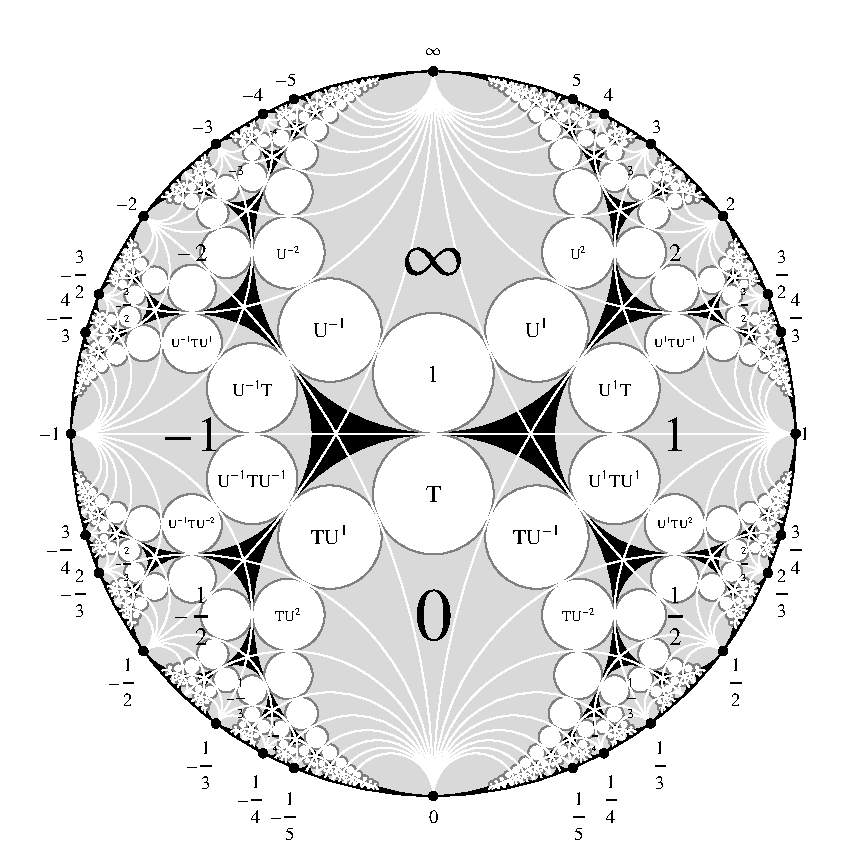
\includegraphics[width=\textwidth]{figures/ford-disks}
\caption{Todo.}
\label{fig_FordDisks}
\end{figure}
Looking at the modular tessellation, Figure~\ref{fig_ModularTiling}, we see that the images of the indisk $\Indisk$ of the fundamental region $\FunDom$ 
have a natural one-to-one correspondence to modular transformations, \ie the disk $A\Indisk$ can be considered as a graphical representative for the modular transformation $A$. 

The question arises, if there is such a visual and clear representation also for left cosets of $\langle U \rangle$ in $\PSL{\Z}$. Indeed, we can see in Figure~\ref{fig_FordDisks}, depicting the modular tessellation under the modified Cayley transform, that the disks $U^k\Indisk$, $k \in \Z$ form a ``generalized ring'' which asymptotically approaches the point $\infty$. We can enclose this ring in a generalized disk -- in Figure~\ref{fig_FordDisks}, this enclosing disk is shown in light gray and is labeled with ``$\infty$''.
\begin{definition}
\label{dfn_FordDisk}
\index{Ford disk}
The unique (open) g-disk $\Forddisk_\infty$ containing all the disks $U^k\Indisk$, $k \in \Z$, in its interior and being tangent to each of them is called the \emph{Ford disk at $\infty$}. It contains all points $z \in \C$ with $\Im{z} > 1$. Its defining matrix is given by
\begin{equation}
\label{eqn_FordDisk}
\Forddisk = \mat{0}{-\ii}{\ii}{2}.
\end{equation}
For a modular transformation $A = \smallmat{a}{b}{c}{d} \in \PSL{\Z}$, the image of $\Forddisk_\infty$ under $A$ is called the \emph{Ford disk at $\frac{a}{c}$}, $\Forddisk_{\frac{a}{c}} := A\Forddisk_\infty$.
\end{definition}

The above definition as well as the bijective correspondence between left cosets of $\langle U \rangle$ in $\PSL{\Z}$ and the extended rational numbers $\EQ$ (Lemma~\ref{lem_MapCosetToEQBijective}) will get much clearer if we again look at Figure~\ref{fig_FordDisks}: We can see that every Ford disk $\Forddisk_r$ (the disk in light gray labeled with $r$), ``touches'' the extended real axis $\R_\infty := \R \cup \{\infty\}$ (appearing as unit circle under the modified Cayley transform) exactly in the point $r$, that is
\begin{equation*}
\topcl{\Forddisk_r} \cap \R_\infty = \{r\} \quad \text{for all } r \in \EQ.
\end{equation*}
For the seeing the relation of Ford disks to left costets of $\langle U \rangle$ in $\PSL{\Z}$, first observe that the Ford disk $\Forddisk_\infty$ contains all the indisks $U^k \Indisk$, $k \in \Z$. We may notate this fact concisely as $\langle U \rangle \Indisk \subseteq \Forddisk_\infty$. In this sense, we can consider $\Forddisk_\infty$ as a graphical representative for the subgroup $\langle U \rangle$ of $\PSL{\Z}$. Clearly every Ford disk $\Forddisk_r$ is the image of $\Forddisk_\infty$ under some transformation $A \in \PSL{\Z}$ (which can be found using Corollary~\ref{cor_ConFracModTrans}), \ie $A\Forddisk_\infty = \Forddisk_r$. Consequently $A \langle U \rangle \Indisk \subseteq \Forddisk_r$ and we can therefore consider $\Forddisk_r$ as graphical representative for the coset $A \langle U \rangle$.

\begin{figure}
\centering
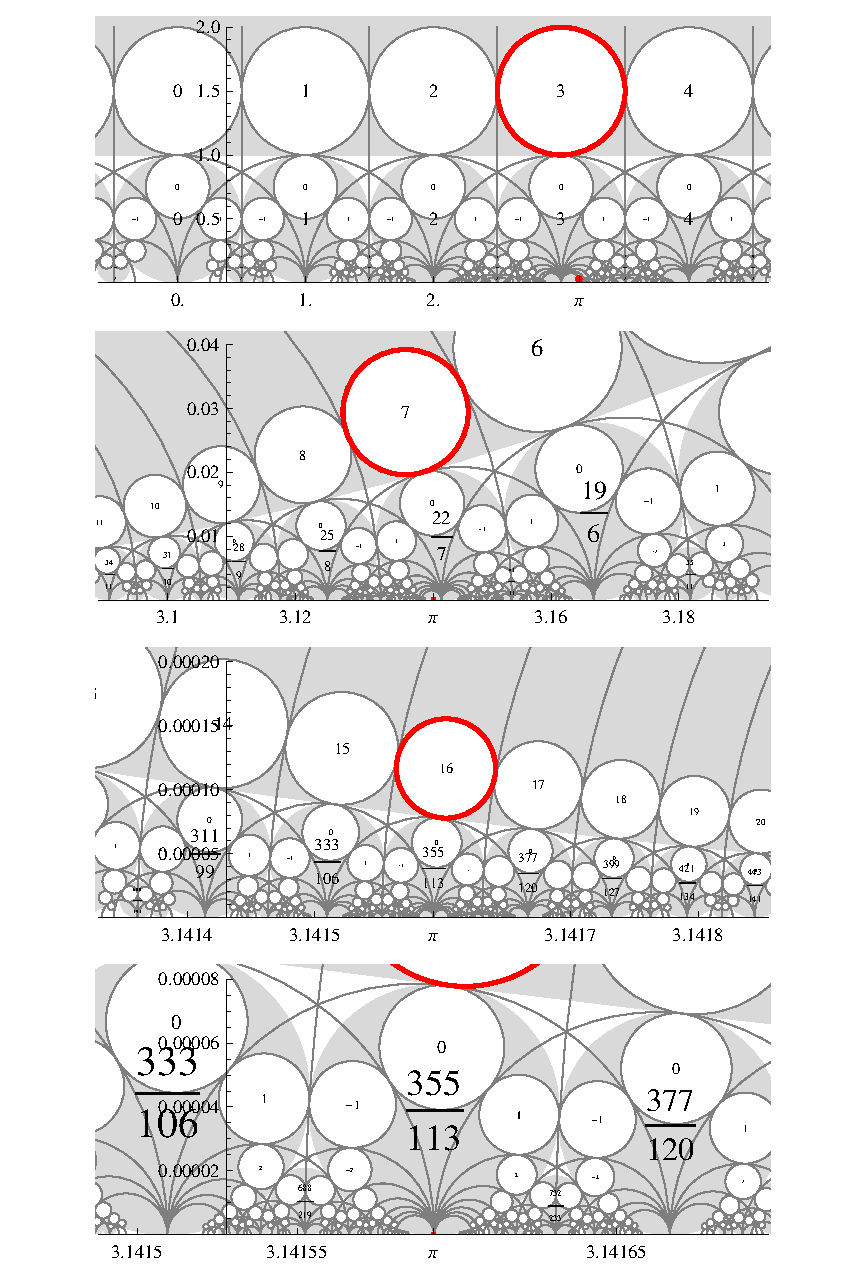
\includegraphics[width=\textwidth]{figures/cont-frac-pi}
\caption{$\pi = \frac{355}{113}$ -- well, almost.}
\label{fig_ContFracPi}
\end{figure}

\todo{19}{The modular group and ford circles}
